\documentclass[sigplan]{acmart}

\usepackage{booktabs} % For formal tables
\usepackage{graphicx,hyperref}
\usepackage{float}
\usepackage{proof,tikz}
\usepackage{amssymb,amsthm,stmaryrd}


% Copyright
%\setcopyright{none}
%\setcopyright{acmcopyright}
%\setcopyright{acmlicensed}
\setcopyright{rightsretained}
%\setcopyright{usgov}
%\setcopyright{usgovmixed}
%\setcopyright{cagov}
%\setcopyright{cagovmixed}


% DOI
\acmDOI{10.475/123_4}

% ISBN
\acmISBN{123-4567-24-567/08/06}

%Conference
\acmConference[SBLP2018]{XXII BRAZILIAN SYMPOSIUM ON PROGRAMMING LANGUAGES}{September 17--21, 2018}{S\~ao Carlos}
\acmYear{2018}
\copyrightyear{2018}

%\acmPrice{15.00}

%\acmBadgeL[http://ctuning.org/ae/ppopp2016.html]{ae-logo}
%\acmBadgeR[http://ctuning.org/ae/ppopp2016.html]{ae-logo}


%% ODER: format ==         = "\mathrel{==}"
%% ODER: format /=         = "\neq "
%
%
\makeatletter
\@ifundefined{lhs2tex.lhs2tex.sty.read}%
  {\@namedef{lhs2tex.lhs2tex.sty.read}{}%
   \newcommand\SkipToFmtEnd{}%
   \newcommand\EndFmtInput{}%
   \long\def\SkipToFmtEnd#1\EndFmtInput{}%
  }\SkipToFmtEnd

\newcommand\ReadOnlyOnce[1]{\@ifundefined{#1}{\@namedef{#1}{}}\SkipToFmtEnd}
\usepackage{amstext}
\usepackage{amssymb}
\usepackage{stmaryrd}
\DeclareFontFamily{OT1}{cmtex}{}
\DeclareFontShape{OT1}{cmtex}{m}{n}
  {<5><6><7><8>cmtex8
   <9>cmtex9
   <10><10.95><12><14.4><17.28><20.74><24.88>cmtex10}{}
\DeclareFontShape{OT1}{cmtex}{m}{it}
  {<-> ssub * cmtt/m/it}{}
\newcommand{\texfamily}{\fontfamily{cmtex}\selectfont}
\DeclareFontShape{OT1}{cmtt}{bx}{n}
  {<5><6><7><8>cmtt8
   <9>cmbtt9
   <10><10.95><12><14.4><17.28><20.74><24.88>cmbtt10}{}
\DeclareFontShape{OT1}{cmtex}{bx}{n}
  {<-> ssub * cmtt/bx/n}{}
\newcommand{\tex}[1]{\text{\texfamily#1}}	% NEU

\newcommand{\Sp}{\hskip.33334em\relax}


\newcommand{\Conid}[1]{\mathit{#1}}
\newcommand{\Varid}[1]{\mathit{#1}}
\newcommand{\anonymous}{\kern0.06em \vbox{\hrule\@width.5em}}
\newcommand{\plus}{\mathbin{+\!\!\!+}}
\newcommand{\bind}{\mathbin{>\!\!\!>\mkern-6.7mu=}}
\newcommand{\rbind}{\mathbin{=\mkern-6.7mu<\!\!\!<}}% suggested by Neil Mitchell
\newcommand{\sequ}{\mathbin{>\!\!\!>}}
\renewcommand{\leq}{\leqslant}
\renewcommand{\geq}{\geqslant}
\usepackage{polytable}

%mathindent has to be defined
\@ifundefined{mathindent}%
  {\newdimen\mathindent\mathindent\leftmargini}%
  {}%

\def\resethooks{%
  \global\let\SaveRestoreHook\empty
  \global\let\ColumnHook\empty}
\newcommand*{\savecolumns}[1][default]%
  {\g@addto@macro\SaveRestoreHook{\savecolumns[#1]}}
\newcommand*{\restorecolumns}[1][default]%
  {\g@addto@macro\SaveRestoreHook{\restorecolumns[#1]}}
\newcommand*{\aligncolumn}[2]%
  {\g@addto@macro\ColumnHook{\column{#1}{#2}}}

\resethooks

\newcommand{\onelinecommentchars}{\quad-{}- }
\newcommand{\commentbeginchars}{\enskip\{-}
\newcommand{\commentendchars}{-\}\enskip}

\newcommand{\visiblecomments}{%
  \let\onelinecomment=\onelinecommentchars
  \let\commentbegin=\commentbeginchars
  \let\commentend=\commentendchars}

\newcommand{\invisiblecomments}{%
  \let\onelinecomment=\empty
  \let\commentbegin=\empty
  \let\commentend=\empty}

\visiblecomments

\newlength{\blanklineskip}
\setlength{\blanklineskip}{0.66084ex}

\newcommand{\hsindent}[1]{\quad}% default is fixed indentation
\let\hspre\empty
\let\hspost\empty
\newcommand{\NB}{\textbf{NB}}
\newcommand{\Todo}[1]{$\langle$\textbf{To do:}~#1$\rangle$}

\EndFmtInput
\makeatother
%
%
%
%
%
%
% This package provides two environments suitable to take the place
% of hscode, called "plainhscode" and "arrayhscode". 
%
% The plain environment surrounds each code block by vertical space,
% and it uses \abovedisplayskip and \belowdisplayskip to get spacing
% similar to formulas. Note that if these dimensions are changed,
% the spacing around displayed math formulas changes as well.
% All code is indented using \leftskip.
%
% Changed 19.08.2004 to reflect changes in colorcode. Should work with
% CodeGroup.sty.
%
\ReadOnlyOnce{polycode.fmt}%
\makeatletter

\newcommand{\hsnewpar}[1]%
  {{\parskip=0pt\parindent=0pt\par\vskip #1\noindent}}

% can be used, for instance, to redefine the code size, by setting the
% command to \small or something alike
\newcommand{\hscodestyle}{}

% The command \sethscode can be used to switch the code formatting
% behaviour by mapping the hscode environment in the subst directive
% to a new LaTeX environment.

\newcommand{\sethscode}[1]%
  {\expandafter\let\expandafter\hscode\csname #1\endcsname
   \expandafter\let\expandafter\endhscode\csname end#1\endcsname}

% "compatibility" mode restores the non-polycode.fmt layout.

\newenvironment{compathscode}%
  {\par\noindent
   \advance\leftskip\mathindent
   \hscodestyle
   \let\\=\@normalcr
   \let\hspre\(\let\hspost\)%
   \pboxed}%
  {\endpboxed\)%
   \par\noindent
   \ignorespacesafterend}

\newcommand{\compaths}{\sethscode{compathscode}}

% "plain" mode is the proposed default.
% It should now work with \centering.
% This required some changes. The old version
% is still available for reference as oldplainhscode.

\newenvironment{plainhscode}%
  {\hsnewpar\abovedisplayskip
   \advance\leftskip\mathindent
   \hscodestyle
   \let\hspre\(\let\hspost\)%
   \pboxed}%
  {\endpboxed%
   \hsnewpar\belowdisplayskip
   \ignorespacesafterend}

\newenvironment{oldplainhscode}%
  {\hsnewpar\abovedisplayskip
   \advance\leftskip\mathindent
   \hscodestyle
   \let\\=\@normalcr
   \(\pboxed}%
  {\endpboxed\)%
   \hsnewpar\belowdisplayskip
   \ignorespacesafterend}

% Here, we make plainhscode the default environment.

\newcommand{\plainhs}{\sethscode{plainhscode}}
\newcommand{\oldplainhs}{\sethscode{oldplainhscode}}
\plainhs

% The arrayhscode is like plain, but makes use of polytable's
% parray environment which disallows page breaks in code blocks.

\newenvironment{arrayhscode}%
  {\hsnewpar\abovedisplayskip
   \advance\leftskip\mathindent
   \hscodestyle
   \let\\=\@normalcr
   \(\parray}%
  {\endparray\)%
   \hsnewpar\belowdisplayskip
   \ignorespacesafterend}

\newcommand{\arrayhs}{\sethscode{arrayhscode}}

% The mathhscode environment also makes use of polytable's parray 
% environment. It is supposed to be used only inside math mode 
% (I used it to typeset the type rules in my thesis).

\newenvironment{mathhscode}%
  {\parray}{\endparray}

\newcommand{\mathhs}{\sethscode{mathhscode}}

% texths is similar to mathhs, but works in text mode.

\newenvironment{texthscode}%
  {\(\parray}{\endparray\)}

\newcommand{\texths}{\sethscode{texthscode}}

% The framed environment places code in a framed box.

\def\codeframewidth{\arrayrulewidth}
\RequirePackage{calc}

\newenvironment{framedhscode}%
  {\parskip=\abovedisplayskip\par\noindent
   \hscodestyle
   \arrayrulewidth=\codeframewidth
   \tabular{@{}|p{\linewidth-2\arraycolsep-2\arrayrulewidth-2pt}|@{}}%
   \hline\framedhslinecorrect\\{-1.5ex}%
   \let\endoflinesave=\\
   \let\\=\@normalcr
   \(\pboxed}%
  {\endpboxed\)%
   \framedhslinecorrect\endoflinesave{.5ex}\hline
   \endtabular
   \parskip=\belowdisplayskip\par\noindent
   \ignorespacesafterend}

\newcommand{\framedhslinecorrect}[2]%
  {#1[#2]}

\newcommand{\framedhs}{\sethscode{framedhscode}}

% The inlinehscode environment is an experimental environment
% that can be used to typeset displayed code inline.

\newenvironment{inlinehscode}%
  {\(\def\column##1##2{}%
   \let\>\undefined\let\<\undefined\let\\\undefined
   \newcommand\>[1][]{}\newcommand\<[1][]{}\newcommand\\[1][]{}%
   \def\fromto##1##2##3{##3}%
   \def\nextline{}}{\) }%

\newcommand{\inlinehs}{\sethscode{inlinehscode}}

% The joincode environment is a separate environment that
% can be used to surround and thereby connect multiple code
% blocks.

\newenvironment{joincode}%
  {\let\orighscode=\hscode
   \let\origendhscode=\endhscode
   \def\endhscode{\def\hscode{\endgroup\def\@currenvir{hscode}\\}\begingroup}
   %\let\SaveRestoreHook=\empty
   %\let\ColumnHook=\empty
   %\let\resethooks=\empty
   \orighscode\def\hscode{\endgroup\def\@currenvir{hscode}}}%
  {\origendhscode
   \global\let\hscode=\orighscode
   \global\let\endhscode=\origendhscode}%

\makeatother
\EndFmtInput
%

\DeclareMathAlphabet{\mathkw}{OT1}{cmss}{bx}{n}

\usetikzlibrary{automata}
\usetikzlibrary{shapes}
\usetikzlibrary{backgrounds}
\usetikzlibrary{positioning}

\newtheorem{Lemma}{Lemma}
\newtheorem{Theorem}{Theorem}
\theoremstyle{definition}
\newtheorem{Example}{Example}

\newcommand{\sembrackets}[1]{\ensuremath{\llbracket #1 \rrbracket}}

\usepackage{color}
\newcommand{\redFG}[1]{\textcolor[rgb]{0.6,0,0}{#1}}
\newcommand{\greenFG}[1]{\textcolor[rgb]{0,0.4,0}{#1}}
\newcommand{\blueFG}[1]{\textcolor[rgb]{0,0,0.8}{#1}}
\newcommand{\orangeFG}[1]{\textcolor[rgb]{0.8,0.4,0}{#1}}
\newcommand{\purpleFG}[1]{\textcolor[rgb]{0.4,0,0.4}{#1}}
\newcommand{\yellowFG}[1]{\textcolor{yellow}{#1}}
\newcommand{\brownFG}[1]{\textcolor[rgb]{0.5,0.2,0.2}{#1}}
\newcommand{\blackFG}[1]{\textcolor[rgb]{0,0,0}{#1}}
\newcommand{\whiteFG}[1]{\textcolor[rgb]{1,1,1}{#1}}
\newcommand{\yellowBG}[1]{\colorbox[rgb]{1,1,0.2}{#1}}
\newcommand{\brownBG}[1]{\colorbox[rgb]{1.0,0.7,0.4}{#1}}

\newcommand{\ColourStuff}{
  \newcommand{\red}{\redFG}
  \newcommand{\green}{\greenFG}
  \newcommand{\blue}{\blueFG}
  \newcommand{\orange}{\orangeFG}
  \newcommand{\purple}{\purpleFG}
  \newcommand{\yellow}{\yellowFG}
  \newcommand{\brown}{\brownFG}
  \newcommand{\black}{\blackFG}
  \newcommand{\white}{\whiteFG}
}

\newcommand{\MonochromeStuff}{
  \newcommand{\red}{\blackFG}
  \newcommand{\green}{\blackFG}
  \newcommand{\blue}{\blackFG}
  \newcommand{\orange}{\blackFG}
  \newcommand{\purple}{\blackFG}
  \newcommand{\yellow}{\blackFG}
  \newcommand{\brown}{\blackFG}
  \newcommand{\black}{\blackFG}
  \newcommand{\white}{\blackFG}
}

\ColourStuff

\newcommand{\D}[1]{\blue{\mathsf{#1}}}
\newcommand{\C}[1]{\red{\mathsf{#1}}}
\newcommand{\F}[1]{\green{\mathsf{#1}}}
\newcommand{\V}[1]{\black{\mathsf{#1}}}
\newcommand{\TC}[1]{\purple{\mathsf{#1}}}


\newcommand{\conf}[1]{\ensuremath{\langle #1 \rangle}}

\begin{document}

\title{Towards certified virtual machine-based regular expression parsing}

\author{Thales Ant\^onio Delfino}
\affiliation{
  \institution{Universidade Federal de Ouro Preto}
  \city{Ouro Preto}
  \state{Minas Gerais}
  \country{Brazil}
}
\author{Rodrigo Ribeiro}
\affiliation{
  \institution{Universidade Federal de Ouro Preto}
  \city{Ouro Preto}
  \state{Minas Gerais}
  \country{Brazil}
}
\begin{abstract}
Regular expressions (REs) are pervasive in computing. We use REs in text editors, string search tools
(like GNU-Grep) and lexical analysers generators. Most of these tools rely on converting regular
expressions to its corresponding finite state machine or use REs derivatives for directly parse an
input string. In this work, we want to investigate the suitability of another approach: instead of
using derivatives or generate a finite state machine for a given RE, we will develop a virtual machine
(VM) for parsing regular languages, in such a way that a RE is merely a program executed by the VM
over the input string. We developed a prototype implementation in Haskell, test it using QuickCheck and
provide proof sketches of its correctness with respect to RE standard inductive semantics.
\end{abstract}

%
% The code below should be generated by the tool at
% http://dl.acm.org/ccs.cfm
% Please copy and paste the code instead of the example below.
%
\begin{CCSXML}\begin{hscode}\SaveRestoreHook
\column{B}{@{}>{\hspre}l<{\hspost}@{}}%
\column{E}{@{}>{\hspre}l<{\hspost}@{}}%
\>[B]{}\V{ccs2012}\mathbin{>}{}\<[E]%
\\
\>[B]{}\V{concept}\mathbin{>}{}\<[E]%
\\
\>[B]{}\V{concept\char95 id}\mathbin{>}\C{10003752.10003766}\mathbin{\circ}\C{10003776}\mathbin{</}\V{concept\char95 id}\mathbin{>}{}\<[E]%
\\
\>[B]{}\V{concept\char95 desc}\mathbin{>}\V{Theory}\;\mathkw{of}\;\V{computation}\mathord{\sim}\V{Regular}\;\V{languages}\mathbin{</}\V{concept\char95 desc}\mathbin{>}{}\<[E]%
\\
\>[B]{}\V{concept\char95 significance}\mathbin{>}\C{500}\mathbin{</}\V{concept\char95 significance}\mathbin{>}{}\<[E]%
\\
\>[B]{}\mathbin{/}\V{concept}\mathbin{>}{}\<[E]%
\\
\>[B]{}\V{concept}\mathbin{>}{}\<[E]%
\\
\>[B]{}\V{concept\char95 id}\mathbin{>}\C{10003752.10010124}\mathbin{\circ}\C{10010131.10010134}\mathbin{</}\V{concept\char95 id}\mathbin{>}{}\<[E]%
\\
\>[B]{}\V{concept\char95 desc}\mathbin{>}\V{Theory}\;\mathkw{of}\;\V{computation}\mathord{\sim}\V{Operational}\;\V{semantics}\mathbin{</}\V{concept\char95 desc}\mathbin{>}{}\<[E]%
\\
\>[B]{}\V{concept\char95 significance}\mathbin{>}\C{500}\mathbin{</}\V{concept\char95 significance}\mathbin{>}{}\<[E]%
\\
\>[B]{}\mathbin{/}\V{concept}\mathbin{>}{}\<[E]%
\\
\>[B]{}\mathbin{/}\V{ccs2012}\mathbin{>}{}\<[E]%
\ColumnHook
\end{hscode}\resethooks
\end{CCSXML}

\ccsdesc[500]{Theory of computation~Regular languages}
\ccsdesc[500]{Theory of computation~Operational semantics}
% We no longer use \terms command
%\terms{Theory}

\keywords{Regular Expressions, Parsing, Virtual Machines, Operational semantics}

\maketitle


\section{Introduction}

We name parsing the process of analyzing if a sequence of symbols matches a given set of rules.
Such rules are usually specified in a formal notation, like a grammar. If a string can be obtained
from those rules, we have success: we can build some evidence that the input is in the language
described by the underlying formalism. Otherwise, we have a failure: no such evidence exists.

In this work, we focus on the parsing problem for regular expressions (REs), which are an algebraic
and compact way of defining regular languages (RLs), i.e. languages that can be recognized by
(non-)deterministic finite automata and equivalent formalisms. REs are widely used in string search
tools, lexical analyser generators and XML schema languages \cite{Frisch2004}. Since RE parsing
is pervasive in computing, its correctness is crucial and is the subject of study of several
recent research works (e.g ~\cite{Firsov13,Ribeiro2017,Lopes2016,Asperti10}).

Approaches for RE parsing can use representations of finite state machines (e.g.~\cite{Firsov13}),
derivatives (e.g.~\cite{Ribeiro2017,Lopes2016}) or the so-called pointed RE's or its
variants~\cite{Asperti10,Fischer2010}. Another approach for parsing is based on the so-called
parsing machines, which dates back to 70's with Knuth's work
on top-down syntax analysis for context-free languages~\cite{Knuth71}. Recently, some works
tried to revive the use of such machines for parsing: Cox~\cite{Cox2009} defined a VM
for which a RE can be seen as ``high-level programs'' that can be compiled to a sequence of
such VM instructions and Lua library LPEG~\cite{Ierusalimschy2009} defines a VM whose instruction
set can be used to compile Parser Expressions Grammars (PEGs)~\cite{Ford04}. Such renewed research
interest is motivated by the fact that is possible to include new features by just adding and
implementing new machine instructions.

Since LPEG VM is designed with PEGs in mind, it is not appropriate for RE parsing, since the ``star''
operator for PEGs has a greedy semantics which differs from the conventional RE semantics for this operator. Also, Cox's work
on VM-based RE parsing has problems. First, it is poorly specified: both the VM semantics and the RE
compilation process are described only informally and no correctness guarantees is even mentioned. Second,
it does not provide an evidence for matching, which could be used to characterize a disambiguation strategy, like
Greedy~\cite{Frisch2004} and POSIX~\cite{Sulzmann14}. To the best of our knowledge, no previous work
has formally defined a VM for RE parsing that produces evidence (parse trees) for successul matches.
The objective of this work is to give a first step in filling this gap. More specifically, we are interested in formally
specify, implement and test the correctness of a VM based small-step semantics for RE parsing which produces bit-codes as
a memory efficient representation of parse-trees. As pointed by~\cite{Lasse2011}, bit-codes are useful because they
are not only smaller than the parse tree, but also smaller than the string being parsed and they can be combined with methods
for text compression. We leave the task of proving that our VM follows a specific disambiguation
strategy to future work.

Our contributions are:

\begin{itemize}
  \item We present a small-step semantics for RE inspired by  Thompson's NFA\footnote{Non-deterministic finite automata.}
        construction~\cite{Thompson1968}. The main novelty of this presentation is
        the use of data-type derivatives, a well-known concept in functional programming community, to represent
        the context in which the current RE being evaluated occur. We show informal proofs\footnote{By ``informal proofs'' we
        mean proofs that are not mechanized in a proof-assistant. Due to space reasons, proofs of the relevant theorems are omitted from this
        version. Detailed proofs can be found in the accompanying technical report avaliable on-line~\cite{regexvm-rep}.} that our semantics
        is sound and complete with respect to RE inductive semantics.
  \item We describe a prototype implementation of our semantics in Haskell and use QuickCheck~\cite{Claessen2000} to test our semantics
        against a simple implementation of RE parsing, presented in~\cite{Fischer2010}, which we conjecture that is correct.
        Our test cases cover both accepted and rejected strings for randomly generated REs.
  \item We show how our proposed semantics can produce bit codes that denote parse trees~\cite{Lasse2011} and test that
        such generated codes correspond to valid parsing evidence using QuickCheck.
\end{itemize}

We are aware that using automated testing is not sufficient to ensure correctness, but it can expose bugs before using more formal approaches,
like formalizing our algorithm in a proof assistant. Such semantic prototyping step is crucial since it can avoid proof attempts that are
doomed to fail due to incorrect definitions. The project's on-line repository~\cite{regexvm-rep} contains the partial Coq formalization of
our semantics. Currently, we have formalized the semantics and its interpreter function. The Coq proof that the proposed small-step semantics
is equivalent to the usual inductive RE semantics is under development.

The rest of this paper is organized as follows. Section~\ref{section:background} presents some background concepts on RE and
data type derivatives that will be used in our semantics. Our operational semantics for RE parsing and its theoretical properties
are described in Section~\ref{section:semantics}. Our prototype implementation and the QuickCheck test suit used to validate
it are presented in Section~\ref{section:implementation}. Section~\ref{section:related} discuss related work and
Section~\ref{section:conclusion} concludes.

We assume that the reader knows the Haskell programming language, specially the list monad and how it can be used
to model non-determinism.  Good introductions to Haskell are available elsewhere~\cite{Lipovaca2011}.
All source code produced, including the literate Haskell source of this
article (which can be preprocessed using lhs2\TeX~\cite{Loh2005}), instructions on how to build it and reproduce the developed
test suit are avaliable on-line~\cite{regexvm-rep}.

\section{Background}\label{section:background}

\subsection{Regular expressions: syntax and semantics}

REs are defined with respect to a given alphabet. Formally, the following context-free
grammar defines RE syntax:
\[
e ::= \emptyset\,\mid\,\epsilon\,\mid\,a\,\mid\,e\,e\,\mid\,e+e\,\mid\,e^{\star}
\]
Meta-variable $e$ will denote an arbitrary RE and $a$ an
arbitrary alphabet symbol. As usual, all meta-variables can appear primed or subscripted.
In our Haskell implementation, we represent alphabet symbols using type \ensuremath{\D{Char}}.


\begin{hscode}\SaveRestoreHook
\column{B}{@{}>{\hspre}l<{\hspost}@{}}%
\column{3}{@{}>{\hspre}l<{\hspost}@{}}%
\column{E}{@{}>{\hspre}l<{\hspost}@{}}%
\>[B]{}\mathkw{data}\;\D{Regex}\mathrel{=}\C{\emptyset}\mid \C{\epsilon}\mid \C{Chr}\;\D{Char}\mid \D{Regex}\C{\:\bullet\:}\D{Regex}{}\<[E]%
\\
\>[B]{}\hsindent{3}{}\<[3]%
\>[3]{}\mid \D{Regex}\C{\:+\:}\D{Regex}\mid \C{Star}\;\D{Regex}{}\<[E]%
\ColumnHook
\end{hscode}\resethooks

Constructors \ensuremath{\C{\emptyset}} and \ensuremath{\C{\epsilon}} denote respectively the
empty set ($\emptyset$) and the empty string ($\epsilon$) REs. Alphabet
symbols are constructed by using the \ensuremath{\C{Chr}} constructor. Bigger REs are
built using concatenation (\ensuremath{\C{\:\bullet\:}}), union (\ensuremath{\C{\:+\:}}) and
Kleene star (\ensuremath{\C{Star}}).

\newcommand{\Eps}{\textit{Eps}}
\newcommand{\Chr}{\textit{Chr}}
\newcommand{\Catt}{\textit{Cat}}
\newcommand{\Left}{\textit{Left}}
\newcommand{\Right}{\textit{Right}}
\newcommand{\StarBase}{\textit{StarBase}}
\newcommand{\StarRec}{\textit{StarRec}}

Following common practice~\cite{Lopes2016,Ribeiro2017,Rathnayake2011}, we adopt an inductive
characterization of RE membership semantics. We let judgement $s \in \sembrackets{e}$ denote
that string $s$ is in the language denoted by RE $e$.

\begin{figure}[h]
  \[
      \begin{array}{cc}
         \infer[_{\{\Eps\}}]
               {\epsilon \in \sembrackets{\epsilon}}{} &
         \infer[_{\{Chr\}}]
               {a \in \sembrackets{a}}{a \in \Sigma} \\ \\
         \infer[_{\{\Left\}}]
               {s \in \sembrackets{e + e'}}{s \in \sembrackets{e}} &
         \infer[_{\{\Right\}}]
               {s' \in \sembrackets{e + e'}}{s' \in \sembrackets{e'}} \\ \\
         \infer[_{\{\StarBase\}}]
               {\epsilon \in \sembrackets{e^\star}}{} &
         \infer[_{\{\StarRec\}}]
               {ss' \in \sembrackets{e^\star}}
               {s \in \sembrackets{e} & s' \in \sembrackets{e^\star}} \\ \\
         \multicolumn{2}{c}{
            \infer[_{\{\Catt\}}]
                  {ss' \in \sembrackets{ee'}}
                  {s \in \sembrackets{e} & s' \in \sembrackets{e'}}
         } \\
      \end{array}
  \]
  \centering
  \caption{RE inductive semantics.}
  \label{figure:resemantics}
\end{figure}

Rule $Eps$ states that the empty string (denoted by the $\epsilon$)
is in the language of RE \ensuremath{\C{\epsilon}}.

For any single character \ensuremath{\V{a}}, the singleton
string \ensuremath{\V{a}} is in the RL
for \ensuremath{\C{Chr}\;\V{a}}. Given membership proofs for REs
\ensuremath{\V{e}} and \ensuremath{\V{e'}}, $s \in \sembrackets{e}$ and $s' \in\sembrackets{e'}$,
rule $Cat$ can be used to build a proof
for the concatenation of these REs.  Rule
\Left~ (\Right) creates a membership proof
for $e + e'$ from a proof for $e$ ($e'$). Semantics for Kleene star
is built using the following well known equivalence of REs: $e^\star
= \epsilon + e\,e^\star$.

We say that a RE $e$ is \emph{problematic}
if $e = e'^\star$ and $\epsilon \in \sembrackets{e'}$~\cite{Frisch2004}.
In this work, we limit our attention to non-problematic RE's. Our results
can be extended to problematic REs without providing any
new insight~\cite{Lasse2011,Frisch2004}.


\subsection{RE parsing and bit-coded parse trees}

\paragraph{RE parsing.}
One way to represent parsing evidence is to build a tree that denotes
a RE membership proof. Following~\cite{Lasse2011,Frisch2004}, we let
parse trees be terms whose type is underlying RE.

\begin{hscode}\SaveRestoreHook
\column{B}{@{}>{\hspre}l<{\hspost}@{}}%
\column{3}{@{}>{\hspre}l<{\hspost}@{}}%
\column{E}{@{}>{\hspre}l<{\hspost}@{}}%
\>[B]{}\mathkw{data}\;\D{Tree}\mathrel{=}\C{()}\mid \C{Chr}\;\D{Char}\mid \D{Tree}\C{\:\bullet\:}\D{Tree}\mid \C{InL}\;\D{Tree}{}\<[E]%
\\
\>[B]{}\hsindent{3}{}\<[3]%
\>[3]{}\mid \C{InR}\;\D{Tree}\mid \C{List}\;[\mskip1.5mu \D{Tree}\mskip1.5mu]{}\<[E]%
\ColumnHook
\end{hscode}\resethooks

Constructor \ensuremath{\C{()}} denotes a tree for RE \ensuremath{\C{\epsilon}} and \ensuremath{\C{Chr}} is a tree
for a single character RE. Trees for concatenations are pairs,
constructors \ensuremath{\C{InL}} and \ensuremath{\C{InR}} denotes trees for the left and right component
of a choice operator. Finally, a tree for RE $e^\star$ is a list of trees for
RE $e$. This informal relation is specified by the following inductive
relation between parse trees and RE. We let $\vdash t : e$ denote that
$t$ is a parse tree for RE $e$.

\begin{figure}[h]
   \[
       \begin{array}{ccc}
          \infer{\vdash \ensuremath{\C{()}} : \epsilon}{} &
          \infer{\vdash \ensuremath{\C{Chr}\;\V{a}} : a} &
          \infer{\vdash \ensuremath{\C{InL}\;\V{t}} : e + e'}
                {\vdash \ensuremath{\V{t}} : e} \\ \\ \\
          \infer{\vdash \ensuremath{\C{InR}\;\V{t'}} : e + e'}
                {\vdash \ensuremath{\V{t'}} : e'} &
          \infer{\vdash \ensuremath{\V{t}\C{\:\bullet\:}\V{t'}} : e e'}
                {\vdash \ensuremath{\V{t}} : e & \vdash \ensuremath{\V{t'}} : e' } &
          \infer{\vdash \ensuremath{\C{List}\;\V{ts}} : e^\star}
                {\forall \ensuremath{\V{t}}. \ensuremath{\V{t}} \in \ensuremath{\V{ts}} \to \vdash \ensuremath{\V{t}} : e} \\
       \end{array}
   \]
   \centering
   \caption{Parse tree typing relation.}
   \label{figure:parsetreetyping}
\end{figure}


The relation between RE semantics and its parse trees are formalized using the
function \ensuremath{\F{flat}}, which builds the string stored in a
given parse tree. The Haskell implementation of \ensuremath{\F{flat}} is immediate.

\begin{hscode}\SaveRestoreHook
\column{B}{@{}>{\hspre}l<{\hspost}@{}}%
\column{E}{@{}>{\hspre}l<{\hspost}@{}}%
\>[B]{}\F{flat}\mathbin{::}\D{Tree}\to \D{String}{}\<[E]%
\\
\>[B]{}\F{flat}\;\C{()}\mathrel{=}\text{\tt \char34 \char34}{}\<[E]%
\\
\>[B]{}\F{flat}\;(\C{Chr}\;\V{c})\mathrel{=}[\mskip1.5mu \V{c}\mskip1.5mu]{}\<[E]%
\\
\>[B]{}\F{flat}\;(\V{t}\C{\:\bullet\:}\V{t'})\mathrel{=}\F{flat}\;\V{t}\plus \F{flat}\;\V{t'}{}\<[E]%
\\
\>[B]{}\F{flat}\;(\C{InL}\;\V{t})\mathrel{=}\F{flat}\;\V{t}{}\<[E]%
\\
\>[B]{}\F{flat}\;(\C{InR}\;\V{t})\mathrel{=}\F{flat}\;\V{t}{}\<[E]%
\\
\>[B]{}\F{flat}\;(\C{List}\;\V{ts})\mathrel{=}\F{concatMap}\;\F{flat}\;\V{ts}{}\<[E]%
\ColumnHook
\end{hscode}\resethooks

The next theorem, which relates parse tress and RE semantics,
can be proved by an easy induction on the RE semantics derivation.
\begin{Theorem}
   For all $s$ and $e$, if $s \in \sembrackets{e}$ then exists a tree \ensuremath{\V{t}}
   such that \ensuremath{\F{flat}\;\V{t}\mathrel{=}} $s$ and $\vdash \ensuremath{\V{t}} : e$.
\end{Theorem}

\paragraph{Bit-coded parse trees.} Nielsen et. al.~\cite{Lasse2011} proposed the
use of bit-marks to register which branch was chosen in a parse tree for union
operator, $+$, and to delimit different matches done by Kleene star expression.
Evidently, not all bit sequences correspond to valid parse trees. Ribeiro et. al.~\cite{Ribeiro2017}
showed an inductively defined relation between valid bit-codes and RE, accordingly to the encoding
proposed by~\cite{Lasse2011}. We let the judgement $bs \rhd e$ denote that the sequence of bits
$bs$ corresponds to a parse-tree for RE $e$.


\begin{figure}[h]
  \[
     \begin{array}{ccc}
        \infer{\ensuremath{[\mskip1.5mu \mskip1.5mu]} \rhd \epsilon}{} &
        \infer{\ensuremath{[\mskip1.5mu \mskip1.5mu]} \rhd a}{}  &
        \infer{\ensuremath{\C{0_b}\mathbin{:}\V{bs}} \rhd e + e'}{\ensuremath{\V{bs}} \rhd e} \\ \\
        \infer{\ensuremath{\C{1_b}\mathbin{:}\V{bs}} \rhd e + e'}{\ensuremath{\V{bs}} \rhd e'} &
        \infer{\ensuremath{\V{bs}\plus \V{bs'}} \rhd e e'}{\ensuremath{\V{bs}} \rhd e & \ensuremath{\V{bs'}} \rhd e'} &
        \infer{\ensuremath{[\mskip1.5mu \C{1_b}\mskip1.5mu]} \rhd e^\star}{} \\ \\
        \multicolumn{3}{c}{
           \infer{\ensuremath{\C{0_b}\mathbin{:}\V{bs}\plus \V{bss}} \rhd e^\star}{\ensuremath{\V{bs}} \rhd e & \ensuremath{\V{bss}} \rhd e^\star}
        }
     \end{array}
  \]
  \centering
  \caption{Typing relation for bit-codes.}
  \label{figure:typing-bitcodes}
\end{figure}

The empty string and single character RE are both represented by empty bit lists. Codes for RE $ee'$ are
built by concatenating codes of $e$ and $e'$. In RE union operator, $+$, the bit \ensuremath{\C{0_b}} marks that the
parse tree for $e + e'$  is built from $e$'s and bit \ensuremath{\C{1_b}} that it is built from $e'$'s. For the Kleene
star, we use bit \ensuremath{\C{1_b}} to denote the parse tree for the empty string and bit \ensuremath{\C{0_b}} to begin matchings of $e$
in a parse tree for $e^\star$.


The relation between a bit-code and its underlying parse tree can be defined using functions
\ensuremath{\F{code}} and \ensuremath{\F{decode}}. Type \ensuremath{\D{Code}} used in \ensuremath{\F{code}} and \ensuremath{\F{decode}} definition is just a synonym
for \ensuremath{[\mskip1.5mu \D{Bit}\mskip1.5mu]}. Function \ensuremath{\F{code}} has an immediate definition by recursion on the structure of parse tree.

\begin{hscode}\SaveRestoreHook
\column{B}{@{}>{\hspre}l<{\hspost}@{}}%
\column{E}{@{}>{\hspre}l<{\hspost}@{}}%
\>[B]{}\F{code}\mathbin{::}\D{Tree}\to \D{Regex}\to \D{Code}{}\<[E]%
\\
\>[B]{}\F{code}\;(\C{InL}\;\V{t})\;(\V{e}\C{\:+\:}\anonymous )\mathrel{=}\C{0_b}\mathbin{:}\F{code}\;\V{t}\;\V{e}{}\<[E]%
\\
\>[B]{}\F{code}\;(\C{InR}\;\V{t'})\;(\anonymous \C{\:+\:}\V{e'})\mathrel{=}\C{1_b}\mathbin{:}\F{code}\;\V{t'}\;\V{e'}{}\<[E]%
\\
\>[B]{}\F{code}\;(\C{List}\;\V{ts})\;(\C{Star}\;\V{e})\mathrel{=}\C{0_b}\mathbin{:}\F{codeList}\;\V{ts}\;\V{e}{}\<[E]%
\\
\>[B]{}\F{code}\;(\V{t}\C{\:\bullet\:}\V{t'})\;(\V{e}\C{\:\bullet\:}\V{e'})\mathrel{=}\F{code}\;\V{t}\;\V{e}\plus \F{code}\;\V{t'}\;\V{e'}{}\<[E]%
\\
\>[B]{}\F{code}\;\anonymous \;\anonymous \mathrel{=}[\mskip1.5mu \mskip1.5mu]{}\<[E]%
\\[\blanklineskip]%
\>[B]{}\F{codeList}\mathbin{::}[\mskip1.5mu \D{Tree}\mskip1.5mu]\to \D{Regex}\to \D{Code}{}\<[E]%
\\
\>[B]{}\F{codeList}\;\V{ts}\;\V{e}\mathrel{=}\F{foldr}\;(\lambda \V{t}\;\V{ac}\to \C{0_b}\mathbin{:}\F{code}\;\V{t}\;\V{e}\plus \V{ac})\;[\mskip1.5mu \C{1_b}\mskip1.5mu]\;\V{ts}{}\<[E]%
\ColumnHook
\end{hscode}\resethooks

To define function \ensuremath{\F{decode}}, we need to keep track of the remaining bits to be processed to finish
tree construction. This task is done by an auxiliar definition, \ensuremath{\F{dec}}.

\begin{hscode}\SaveRestoreHook
\column{B}{@{}>{\hspre}l<{\hspost}@{}}%
\column{6}{@{}>{\hspre}l<{\hspost}@{}}%
\column{7}{@{}>{\hspre}l<{\hspost}@{}}%
\column{E}{@{}>{\hspre}l<{\hspost}@{}}%
\>[B]{}\F{dec}\mathbin{::}\D{Regex}\to \D{Code}\to \D{Maybe}\;(\D{Tree},\D{Code}){}\<[E]%
\\
\>[B]{}\F{dec}\;\C{\epsilon}\;\V{bs}\mathrel{=}\F{return}\;(\C{()},\V{bs}){}\<[E]%
\\
\>[B]{}\F{dec}\;(\C{Chr}\;\V{c})\;\V{bs}\mathrel{=}\F{return}\;(\C{Chr}\;\V{c},\V{bs}){}\<[E]%
\\
\>[B]{}\F{dec}\;(\V{e}\C{\:+\:}\anonymous )\;(\C{0_b}\mathbin{:}\V{bs})\mathrel{=}\mathkw{do}{}\<[E]%
\\
\>[B]{}\hsindent{6}{}\<[6]%
\>[6]{}(\V{t},\V{bs1})\leftarrow \F{dec}\;\V{e}\;\V{bs}{}\<[E]%
\\
\>[B]{}\hsindent{6}{}\<[6]%
\>[6]{}\F{return}\;(\C{InL}\;\V{t},\V{bs1}){}\<[E]%
\\
\>[B]{}\F{dec}\;(\anonymous \C{\:+\:}\V{e'})\;(\C{1_b}\mathbin{:}\V{bs})\mathrel{=}\mathkw{do}{}\<[E]%
\\
\>[B]{}\hsindent{6}{}\<[6]%
\>[6]{}(\V{t'},\V{bs1})\leftarrow \F{dec}\;\V{e'}\;\V{bs}{}\<[E]%
\\
\>[B]{}\hsindent{6}{}\<[6]%
\>[6]{}\F{return}\;(\C{InR}\;\V{t'},\V{bs1}){}\<[E]%
\\
\>[B]{}\F{dec}\;(\V{e}\C{\:\bullet\:}\V{e'})\;\V{bs}\mathrel{=}\mathkw{do}{}\<[E]%
\\
\>[B]{}\hsindent{7}{}\<[7]%
\>[7]{}(\V{t},\V{bs1})\leftarrow \F{dec}\;\V{e}\;\V{bs}{}\<[E]%
\\
\>[B]{}\hsindent{7}{}\<[7]%
\>[7]{}(\V{t'},\V{bs'})\leftarrow \F{dec}\;\V{e'}\;\V{bs1}{}\<[E]%
\\
\>[B]{}\hsindent{7}{}\<[7]%
\>[7]{}\F{return}\;(\V{t}\C{\:\bullet\:}\V{t'},\V{bs'}){}\<[E]%
\\
\>[B]{}\F{dec}\;(\C{Star}\;\V{e})\;\V{bs}\mathrel{=}\mathkw{do}{}\<[E]%
\\
\>[B]{}\hsindent{7}{}\<[7]%
\>[7]{}(\V{ts},\V{bs'})\leftarrow \F{decodeList}\;\V{e}\;\V{bs}{}\<[E]%
\\
\>[B]{}\hsindent{7}{}\<[7]%
\>[7]{}\F{return}\;(\C{List}\;\V{ts},\V{bs'}){}\<[E]%
\\
\>[B]{}\F{dec}\;\anonymous \;\anonymous \mathrel{=}\F{fail}\;\text{\tt \char34 invalid~bit~code\char34}{}\<[E]%
\ColumnHook
\end{hscode}\resethooks
For single character and empty string REs, its decoding consists in just building
the tree and leaving the input bit-coded untouched. We build a left tree (using \ensuremath{\C{InL}})
for $e + e'$ if the code starts with bit \ensuremath{\C{0_b}}. A parse tree using constructor \ensuremath{\C{InR}} is built
whenever we find bit \ensuremath{\C{1_b}} for a union RE. Building a tree for concatenation is done by
sequencing the processing of codes for left component of concatenation and starting the
processing of right component with the remaining bits from the processing of the left RE.
\begin{hscode}\SaveRestoreHook
\column{B}{@{}>{\hspre}l<{\hspost}@{}}%
\column{7}{@{}>{\hspre}l<{\hspost}@{}}%
\column{E}{@{}>{\hspre}l<{\hspost}@{}}%
\>[B]{}\F{decodeList}\mathbin{::}\D{Regex}\to \D{Code}\to \D{Maybe}\;([\mskip1.5mu \D{Tree}\mskip1.5mu],\D{Code}){}\<[E]%
\\
\>[B]{}\F{decodeList}\;\anonymous \;[\mskip1.5mu \mskip1.5mu]\mathrel{=}\F{fail}\;\text{\tt \char34 fail~decodeList\char34}{}\<[E]%
\\
\>[B]{}\F{decodeList}\;\anonymous \;(\C{1_b}\mathbin{:}\V{bs})\mathrel{=}\F{return}\;([\mskip1.5mu \mskip1.5mu],\V{bs}){}\<[E]%
\\
\>[B]{}\F{decodeList}\;\V{e}\;(\C{0_b}\mathbin{:}\V{bs})\mathrel{=}\mathkw{do}{}\<[E]%
\\
\>[B]{}\hsindent{7}{}\<[7]%
\>[7]{}(\V{t},\V{be})\leftarrow \F{dec}\;\V{e}\;\V{bs}{}\<[E]%
\\
\>[B]{}\hsindent{7}{}\<[7]%
\>[7]{}(\V{ts},\V{bs'})\leftarrow \F{decodeList}\;\V{e}\;\V{be}{}\<[E]%
\\
\>[B]{}\hsindent{7}{}\<[7]%
\>[7]{}\F{return}\;(\V{t}\mathbin{:}\V{ts},\V{bs'}){}\<[E]%
\ColumnHook
\end{hscode}\resethooks
Function \ensuremath{\F{decodeList}} generate a list of parse trees consuming the bit \ensuremath{\C{0_b}} used
as a separator, and bit \ensuremath{\C{1_b}} which finish the list of parsing results for star operator.

Finally, using \ensuremath{\V{dec}}, the definition of \ensuremath{\F{decode}} is immediate.
\begin{hscode}\SaveRestoreHook
\column{B}{@{}>{\hspre}l<{\hspost}@{}}%
\column{3}{@{}>{\hspre}l<{\hspost}@{}}%
\column{8}{@{}>{\hspre}l<{\hspost}@{}}%
\column{21}{@{}>{\hspre}l<{\hspost}@{}}%
\column{E}{@{}>{\hspre}l<{\hspost}@{}}%
\>[B]{}\F{decode}\mathbin{::}\D{Regex}\to \D{Code}\to \D{Maybe}\;\D{Tree}{}\<[E]%
\\
\>[B]{}\F{decode}\;\V{e}\;\V{bs}{}\<[E]%
\\
\>[B]{}\hsindent{3}{}\<[3]%
\>[3]{}\mathrel{=}\mathkw{case}\;\F{dec}\;\V{e}\;\V{bs}\;\mathkw{of}{}\<[E]%
\\
\>[3]{}\hsindent{5}{}\<[8]%
\>[8]{}\C{Just}\;(\V{t},[\mskip1.5mu \mskip1.5mu])\to \C{Just}\;\V{t}{}\<[E]%
\\
\>[3]{}\hsindent{5}{}\<[8]%
\>[8]{}\anonymous {}\<[21]%
\>[21]{}\to \C{Nothing}{}\<[E]%
\ColumnHook
\end{hscode}\resethooks
The relation between codes and its correspondent parse trees are specified by the next
theorem.
\begin{Theorem}
  Let $t$ be a parse tree such that $\vdash t : e$, for some RE e. Then $\ensuremath{(\F{code}\;\V{t}\;\V{e})} \rhd e$ and
  \ensuremath{\F{decode}\;\V{e}\;(\F{code}\;\V{t}\;\V{e})\mathrel{=}\C{Just}\;\V{t}}.
\end{Theorem}

Next, we review Thompson NFA construction which is similar to the proposed semantics
for RE parsing developed in Section~\ref{section:semantics}.

\subsection{Thompson NFA construction}

The Thompson NFA construction is a classical algorithm for building an equivalent
NFA with $\epsilon$-transitions by induction over the structure of an input RE.
We follow a presentation given in~\cite{Aho1986} where $N(e)$ denotes the NFA
equivalent to RE $e$. The construction proceeds as follows. If $e = \epsilon$,
we can build the following NFA equivalent to $e$.
\begin{center}
  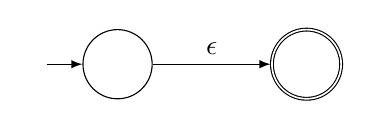
\begin{tikzpicture}[auto, node distance=24mm, initial text=, >=latex]
      \node[state, initial, fill=white]   (q_1) [] {};
      \node[state, accepting, fill=white] (q_2) [right of=q_1] {};

      \path[->] (q_1) edge [] node {$\epsilon$}  (q_2);
  \end{tikzpicture}
\end{center}
If $e = a$, for $a \in \Sigma$, we can make a NFA with a single transition consuming
$a$:
\begin{center}
 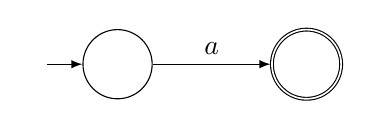
\begin{tikzpicture}[auto, node distance=24mm, initial text=, >=latex]
      \node[state, initial, fill=white]   (q_1) [] {};
      \node[state, accepting, fill=white] (q_2) [right of=q_1] {};

      \path[->] (q_1) edge [] node {$a$}  (q_2);
 \end{tikzpicture}
\end{center}
When $e = e_1 + e_2$, we let $N(e_1)$ be the NFA for $e_1$ and $N(e_2)$ the
NFA for $e_2$. The NFA for $e_1 + e_2$ is built by adding a new initial and accepting
state which can be combined with $N(e_1)$ and $N(e_2)$ using $\epsilon$-transitions as
shown in the next picture.
\begin{center}
    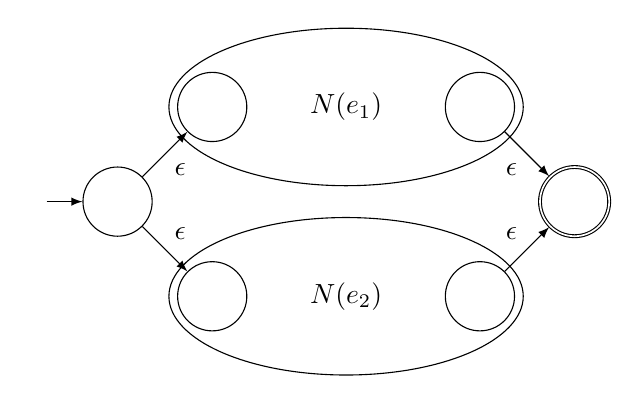
\begin{tikzpicture}[auto, node distance=17mm, initial text=, >=latex]
      \node[state, initial]  (s_i)   []                   {};
      \node[state]        (a_1)   [above right of=s_i] {};
      \node[draw=none,fill=none]            (namea) [right of=a_1] {$N(e_1)$};
      \node[state]         (a_2)   [right of=namea]     {};

      \node[state]        (b_1)   [below right of=s_i] {};
      \node[draw=none]            (nameb) [right of=b_1]           {$N(e_2)$};
      \node[state]         (b_2)   [right of=nameb]     {};

      \node[state, accepting] (s_a)   [below right of=a_2] {};

      \path[->] (s_i) edge [below right] node {$\epsilon$} (a_1)
                      edge [above right] node {$\epsilon$} (b_1)
                (a_2) edge [below left]  node {$\epsilon$} (s_a)
                (b_2) edge []            node {$\epsilon$} (s_a);
      \begin{scope}[on background layer]
        \node[ellipse, draw=black, aspect=5, minimum width=45mm, minimum height=20mm, right of=b_1] {};
        \node[ellipse, draw=black, aspect=5, minimum width=45mm, minimum height=20mm, right of=a_1] {};
      \end{scope}
    \end{tikzpicture}
\end{center}
The NFA for the concatenation $e = e_1e_2$ is built from the NFAs $N(e_1)$ and $N(e_2)$. The accepting
state of $N(e_1e_2)$ will be the accepting state from $N(e_2)$ and the starting state of $N(e_1)$ will be
the initial state of $N(e_1)$.

\begin{center}
    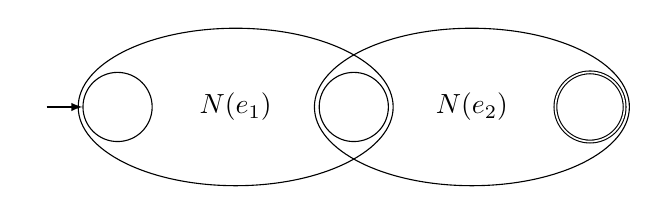
\begin{tikzpicture}[auto,  node distance=15mm, initial text=, >=latex]
      \node[state, initial]   (a_1)   []               {};
      \node[draw=none,fill=none]             (namea) [right of=a_1]   {$N(e_1)$};
      \node[state] (a_2)   [right of=namea] {};

      \node[draw=none]             (nameb) [right of=a_2]   {$N(e_2)$};
      \node[state, accepting]  (b_2)   [right of=nameb] {};

      \begin{scope}[on background layer]
        \node[ellipse, draw=black, aspect=5, minimum width=40mm, minimum height=20mm, right of=a_1] {};
        \node[ellipse, draw=black, aspect=5, minimum width=40mm, minimum height=20mm, right of=a_2] {};
      \end{scope}
    \end{tikzpicture}
\end{center}
Finally, for the Kleene star operator, we built a NFA for the RE $e$, add a new
starting and accepting states and the necessary $\epsilon$ transitions, as shown below.
\begin{center}
    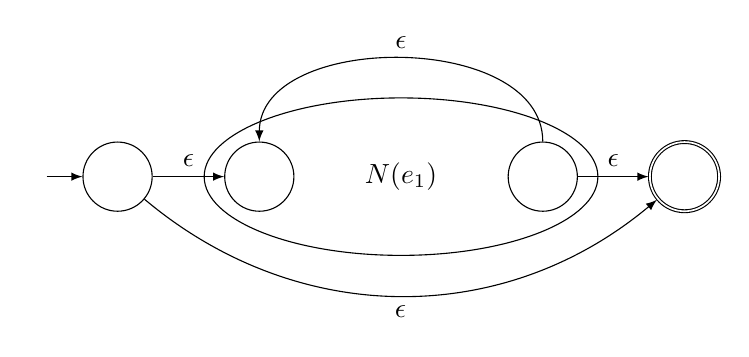
\begin{tikzpicture}[auto, node distance=18mm, initial text=, >=latex]
      \node[state, initial]  (s_i)   []               {};
      \node[state]        (a_1)   [right of=s_i]   {};
      \node[draw=none]            (namea) [right of=a_1]   {$N(e_1)$};
      \node[state]         (a_2)   [right of=namea] {};

      \node[state, accepting] (s_a)   [right of=a_2]   {};

      \path[->] (s_i) edge []                     node {$\epsilon$} (a_1)
                      edge [bend right=40, below] node {$\epsilon$} (s_a)
                (a_2) edge []                     node {$\epsilon$} (s_a)
                      edge [bend right=90, above] node {$\epsilon$} (a_1);
      \begin{scope}[on background layer]
        \node[ellipse, draw=black, aspect=5, minimum width=50mm, minimum height=20mm, right of=a_1] {};
      \end{scope}
    \end{tikzpicture}
\end{center}
Originally, Thompson formulate its construction as a IBM 7094 program~\cite{Thompson1968}. Next we reformulate it as a small-step
operational semantics using contexts, modelled as data-type derivatives for RE, which is the subject of
the next section.

\subsection{Data-type derivatives}

The usage of evaluation contexts is standard in reduction semantics~\cite{Felleisen2009}.
Contexts for evaluating a RE during the parse of a string $s$ can be defined by the following
context-free syntax:
\[E[\,] \to E[\,]+ e\,\mid\,e + E[\,]\,\mid\,E[\,]\,e\,\mid\,e\,E[\,]\,\mid\,\star\]

The semantics of a $E[\,]$ context is a RE with a hole that needs to be ``filled'' to form a
RE. We have two cases for union and concatenation denoting that the hole could be the left
or the right component of such operators. Since the Kleene star has only a recursive occurrence,
it is denoted just as a ``mark'' in context syntax.

Having defined our semantics (Figure~\ref{figure:smallstep}), we have noticed that our RE context syntax is exactly the data type
for \emph{one-hole contexts}, known as derivative of an algebraic data type.
Derivatives where introduced by McBride and its coworkers~\cite{McBride08} as a generalization
of Huet's zippers for a large class of algebraic data types~\cite{AbbottAGM03}. RE contexts are
implemented by the following Haskell data-type:
\begin{hscode}\SaveRestoreHook
\column{B}{@{}>{\hspre}l<{\hspost}@{}}%
\column{3}{@{}>{\hspre}l<{\hspost}@{}}%
\column{E}{@{}>{\hspre}l<{\hspost}@{}}%
\>[B]{}\mathkw{data}\;\D{Hole}\mathrel{=}\C{InChoiceL}\;\D{Regex}\mid \C{InChoiceR}\;\D{Regex}{}\<[E]%
\\
\>[B]{}\hsindent{3}{}\<[3]%
\>[3]{}\mid \C{InCatL}\;\D{Regex}\mid \C{InCatR}\;\D{Regex}\mid \C{InStar}{}\<[E]%
\ColumnHook
\end{hscode}\resethooks
Constructor \ensuremath{\C{InChoiceL}} store the right component of a union RE (similarly for \ensuremath{\C{InChoiceR}}). We need
to store contexts for union because such information is used to allow backtracking in case of failure.
Constructors \ensuremath{\C{InCatL}} and \ensuremath{\C{InCatR}} store the right (left) component of a concatenation and they are
used to store the next subexpresssions that needed to be evaluated during input string parsing.
Finally, \ensuremath{\C{InStar}} marks that we are currently processing an expression with a Kleene star operator.

\section{Proposed semantics}\label{section:semantics}


In this section we present the definition of an operational semantics for RE parsing which is
equivalent to executing the Thompson's construction NFA over the input string. Observe that,
the inductive semantics for RE (Figure~\ref{figure:resemantics}) can be understood as a big-step
operational semantics for RE, since it ignores many details on how should we proceed to match
an input~\cite{Rathnayake2011}.

The semantics is defined as a binary relation between \emph{configurations}, which are 5-uples
$\conf{d,e,c,b,s}$ where:
\begin{itemize}
  \item $d$ is a direction, which specifies if the semantics is starting (denoted by $B$) or
        finishing ($F$) the processing of the current expression $e$.
  \item $e$ is the current expression being evaluated;
  \item $c$ is a context in which $e$ occurs. Contexts are just a list of
        \ensuremath{\D{Hole}} type in our implementation.
  \item $b$ is a bit-code for the current parsing result, in reverse order.
  \item $s$ is the input string currently being processed.
\end{itemize}
Notation $\conf{d,e,c,b,s}\to\conf{d',e',c',b',s'}$ denotes that from
configuration $\conf{d,e,c,b,s}$ we can give a step leading to a new state
$\conf{d',e',c',b',s'}$ using the rules specified in Figure~\ref{figure:smallstep}.

\begin{figure*}[h]
  \[
     \begin{array}{ccc}
        \infer[_{(Eps)}]{\conf{B,\epsilon,c,b,s} \to \conf{F,\epsilon,c,b,s}}{}
        &
        \infer[_{(Chr)}]{\conf{B,a,c,b,a:s} \to \conf{F,a,c,b,s}}{}
        &
        \infer[_{(Left_B)}]{\conf{B,e+e',c,b,s}\to\conf{B,e,c',b',s}}
              {\begin{array}{c}
                 b' = \ensuremath{\C{0_b}} : b\\
                 c' = E[\,]+e' : c \\
               \end{array}}
        \\ \\
        \infer[_{(Right_B)}]{\conf{B,e+e',c,b,s}\to\conf{B,e',c',b',s}}
              {\begin{array}{c}
                 b' = \ensuremath{\C{1_b}} : b\\
                 c' = e + E[\,] : c \\
               \end{array}}
        &
        \infer[_{(Cat_B)}]{\conf{B,ee',c,b,s}\to\conf{B,e,c',b,s}}
              {c' = E[\,]e' : c}
        &
        \infer[_{(Star_1)}]{\conf{B,e^\star,c,b,s}\to\conf{B,e,\star : c, \ensuremath{\C{0_b}} : b, s}}{}
        \\ \\
        \infer[_{(Star_2)}]{\conf{B,e^\star,c,b,s}\to\conf{F,e^\star, c, \ensuremath{\C{1_b}} : b, s}}{}
        &
        \infer[_{(Cat_{EL})}]{\conf{F,e,E[\,]e':c,b,s}\to\conf{B,e',c',b,s}}{c'=eE[\,]:c}
        &
        \infer[_{(Cat_{ER})}]{\conf{F,e',eE[\,]:c,b,s}\to\conf{F,ee',c,b,s}}{}
        \\ \\
        \multicolumn{3}{c}{
            \begin{array}{cc}
               \infer[_{(Left_E)}]{\conf{F,e,c,b,s}\to\conf{F,e+e',c',\ensuremath{\C{0_b}}:b,s}}{c = E[\,]+e' : c'}
            &
               \infer[_{(Right_E)}]{\conf{F,e,c,b,s}\to\conf{F,e+e',c',\ensuremath{\C{1_b}}:b,s}}{c = e + E[\,] : c'}
            \end{array}}
        \\ \\
        \multicolumn{3}{c}{
           \begin{array}{cc}
              \infer[_{(Star_{E1})}]{\conf{F,e,\star:c,b,s}\to\conf{B,e,\star:c,\ensuremath{\C{0_b}}:b,s}}{}
              &
              \infer[_{(Star_{E2})}]{\conf{F,e,\star:c,b,s}\to\conf{F,e^\star,c,\ensuremath{\C{1_b}}:b,s}}{}
           \end{array}
        }
     \end{array}
  \]
  \centering
  \caption{Small-step semantics for RE parsing.}
  \label{figure:smallstep}
\end{figure*}
The rules of the semantics can be divided in two groups: starting rules and finishing rules.
Starting rules deal with configurations with a begin ($B$) direction and denote that we are
beginning the parsing for its RE $e$. Finishing rules use the context to decide how the parsing
for some expression should end. Intuitively, starting rules correspond to transitions entering a
sub-automata of Thompson NFA and finishing rules to transitions exiting a sub-automata.

The meaning of each starting rule is as follows. Rule $\{Eps\}$ specifies that we can mark a state as
finished if it consists of a starting configuration with RE $\epsilon$. We can finish any configuration
for \ensuremath{\C{Chr}\;\V{a}} if it is starting with current string with a leading $a$. Whenever we have a starting configuration
with a choice RE, $e_1 + e_2$, we can non-deterministicaly choose if input string $s$ can be processed by
$e_1$ (rule $Left_B$) or $e_2$ (rule $Right_B$). For beginning configurations with concatenation, we parse
input string using each of its components sequentially. Finally, for starting configurations with a Kleene
star operator, $e^\star$, we can either start the processing of $e$ or finish the processing for $e^\star$.
In all recursive cases for RE, we insert context information in the third component of the resulting
configuration in order to decide how the machine should step after finishing the execution of the RE
currently on focus.

Rule $(Cat_{EL})$ applies to any configuration which is finishing with a left concatenation context ($E[\,]e'$).
In such situation, rule specifies that a computation should continue with $e'$ and push the context $e\,E[\,]$.
We end the computation for a concatenation, whenever we find a context $e\,E[\,]$ in the context component
(rule $(Cat_{ER})$). Finishing a computation for choice consists in just popping its correspondent context,
as done by rules $(Left_E)$ and $(Right_E)$. For the Kleene star operator, we can either finish the computation
by popping the contexts and adding the corresponding \ensuremath{\C{1_b}} to end its matching list or restart with RE $e$ for
another matching over the input string.

The starting state of the semantics is given by the configuration
$\conf{B,e,[],[],s}$ and accepting configurations are $\conf{F,e',[],bs,[]}$, for some RE $e'$ and code $bs$.
Following common practice, we let $\to^\star$ denote the reflexive, transtive closure of the small-step
semantics defined in Figure~\ref{figure:smallstep}.
We say that a string $s$ is accepted by RE $e$ if $\conf{B,e,[],[],s}\to^\star\conf{F,e',[],bs,[]}$.
The next theorem asserts that our semantics is sound and complete with respect to RE
inductive semantics (Figure~\ref{figure:resemantics}).

\begin{Theorem}
   For all strings $s$ and non-problematic REs $e$, $s\in\sembrackets{e}$ if, and only if, $\conf{B,e,[],[],s}\to^\star\conf{F,e',[],b,[]}$ and
   $\conf{F,e',[],b,[]}$ is an accepting configuration.
\end{Theorem}

\section{Implementation details}\label{section:implementation}


In order to implement the small-step semantics of Figure~\ref{figure:smallstep}, we need to represent configurations.
We use type \ensuremath{\D{Conf}} to denote configurations and directions are represented by type \ensuremath{\D{Dir}}, where \ensuremath{\C{Begin}} denote the
starting and \ensuremath{\C{End}} the finishing direction.

\begin{hscode}\SaveRestoreHook
\column{B}{@{}>{\hspre}l<{\hspost}@{}}%
\column{E}{@{}>{\hspre}l<{\hspost}@{}}%
\>[B]{}\mathkw{data}\;\D{Dir}\mathrel{=}\C{Begin}\mid \C{End}{}\<[E]%
\\
\>[B]{}\mathkw{type}\;\D{Conf}\mathrel{=}(\D{Dir},\D{Regex},[\mskip1.5mu \D{Hole}\mskip1.5mu],\D{Code},\D{String}){}\<[E]%
\ColumnHook
\end{hscode}\resethooks

Function \ensuremath{\F{finish}} tests if a configuration is an accepting one.

\begin{hscode}\SaveRestoreHook
\column{B}{@{}>{\hspre}l<{\hspost}@{}}%
\column{E}{@{}>{\hspre}l<{\hspost}@{}}%
\>[B]{}\F{finish}\mathbin{::}\D{Conf}\to \D{Bool}{}\<[E]%
\\
\>[B]{}\F{finish}\;(\C{End},\anonymous ,[\mskip1.5mu \mskip1.5mu],\anonymous ,[\mskip1.5mu \mskip1.5mu])\mathrel{=}\C{True}{}\<[E]%
\\
\>[B]{}\F{finish}\;\anonymous \mathrel{=}\C{False}{}\<[E]%
\ColumnHook
\end{hscode}\resethooks


The small-step semantics is implemented by function \ensuremath{\F{next}}, which returns a list of configurations that can
be reached from a given input configuration. We will begin by explaining the equations that code the set of
starting rules from the small-step semantics. The first alternative

\begin{hscode}\SaveRestoreHook
\column{B}{@{}>{\hspre}l<{\hspost}@{}}%
\column{E}{@{}>{\hspre}l<{\hspost}@{}}%
\>[B]{}\F{next}\mathbin{::}\D{Conf}\to [\mskip1.5mu \D{Conf}\mskip1.5mu]{}\<[E]%
\\
\>[B]{}\F{next}\;(\C{Begin},\C{\epsilon},\V{ctx},\V{bs},\V{s})\mathrel{=}[\mskip1.5mu (\C{End},\C{\epsilon},\V{ctx},\V{bs},\V{s})\mskip1.5mu]{}\<[E]%
\ColumnHook
\end{hscode}\resethooks
implements rule $(Eps)$, which finishes a starting \ensuremath{\D{Conf}} with an \ensuremath{\C{\epsilon}}. Rule $(Chr)$ is implemented by
the following equation
\begin{hscode}\SaveRestoreHook
\column{B}{@{}>{\hspre}l<{\hspost}@{}}%
\column{3}{@{}>{\hspre}l<{\hspost}@{}}%
\column{15}{@{}>{\hspre}l<{\hspost}@{}}%
\column{E}{@{}>{\hspre}l<{\hspost}@{}}%
\>[B]{}\F{next}\;(\C{Begin},\C{Chr}\;\V{c},\V{ctx},\V{bs},\V{a}\mathbin{:}\V{s}){}\<[E]%
\\
\>[B]{}\hsindent{3}{}\<[3]%
\>[3]{}\mid \V{a}\equiv \V{c}\mathrel{=}{}\<[15]%
\>[15]{}[\mskip1.5mu (\C{End},\C{Chr}\;\V{c},\V{ctx},\V{bs},\V{s})\mskip1.5mu]{}\<[E]%
\\
\>[B]{}\hsindent{3}{}\<[3]%
\>[3]{}\mid \F{otherwise}\mathrel{=}[\mskip1.5mu \mskip1.5mu]{}\<[E]%
\ColumnHook
\end{hscode}\resethooks
which consumes input character \ensuremath{\V{a}} if it matches RE \ensuremath{\C{Chr}\;\V{c}}, otherwise it fails by returning an empty list.
For a choice expression, we can use two distinct rules: one for parsing the input using its left component and
another rule for the right. Since both union and Kleene star introduce non-determinism in RE parsing, we can
easily model this using the list monad, by return a list of possible resulting configurations.
\begin{hscode}\SaveRestoreHook
\column{B}{@{}>{\hspre}l<{\hspost}@{}}%
\column{3}{@{}>{\hspre}l<{\hspost}@{}}%
\column{5}{@{}>{\hspre}l<{\hspost}@{}}%
\column{E}{@{}>{\hspre}l<{\hspost}@{}}%
\>[B]{}\F{next}\;(\C{Begin},\V{e}\C{\:+\:}\V{e'},\V{ctx},\V{bs},\V{s}){}\<[E]%
\\
\>[B]{}\hsindent{3}{}\<[3]%
\>[3]{}\mathrel{=}[\mskip1.5mu (\C{Begin},\V{e},\C{InChoiceL}\;\V{e'}\mathbin{:}\V{ctx},\C{0_b}\mathbin{:}\V{bs},\V{s}){}\<[E]%
\\
\>[3]{}\hsindent{2}{}\<[5]%
\>[5]{},(\C{Begin},\V{e'},\C{InChoiceR}\;\V{e}\mathbin{:}\V{ctx},\C{1_b}\mathbin{:}\V{bs},\V{s})\mskip1.5mu]{}\<[E]%
\ColumnHook
\end{hscode}\resethooks
Concatenation just sequences the computation of each of its composing RE.
\begin{hscode}\SaveRestoreHook
\column{B}{@{}>{\hspre}l<{\hspost}@{}}%
\column{3}{@{}>{\hspre}l<{\hspost}@{}}%
\column{E}{@{}>{\hspre}l<{\hspost}@{}}%
\>[B]{}\F{next}\;(\C{Begin},\V{e}\C{\:\bullet\:}\V{e'},\V{ctx},\V{bs},\V{s}){}\<[E]%
\\
\>[B]{}\hsindent{3}{}\<[3]%
\>[3]{}\mathrel{=}[\mskip1.5mu (\C{Begin},\V{e},\C{InCatL}\;\V{e'}\mathbin{:}\V{ctx},\V{bs},\V{s})\mskip1.5mu]{}\<[E]%
\ColumnHook
\end{hscode}\resethooks
For a starting configuration with Kleene star operator, \ensuremath{\C{Star}\;\V{e}}, we can proceed in two ways: by beginning the
parsing of RE \ensuremath{\V{e}} or by finishing the computation for \ensuremath{\C{Star}\;\V{e}} over the input.
\begin{hscode}\SaveRestoreHook
\column{B}{@{}>{\hspre}l<{\hspost}@{}}%
\column{3}{@{}>{\hspre}l<{\hspost}@{}}%
\column{5}{@{}>{\hspre}l<{\hspost}@{}}%
\column{E}{@{}>{\hspre}l<{\hspost}@{}}%
\>[B]{}\F{next}\;(\C{Begin},\C{Star}\;\V{e},\V{ctx},\V{bs},\V{s}){}\<[E]%
\\
\>[B]{}\hsindent{3}{}\<[3]%
\>[3]{}\mathrel{=}[\mskip1.5mu (\C{Begin},\V{e},\C{InStar}\mathbin{:}\V{ctx},\C{0_b}\mathbin{:}\V{bs},\V{s}){}\<[E]%
\\
\>[3]{}\hsindent{2}{}\<[5]%
\>[5]{},(\C{End},(\C{Star}\;\V{e}),\V{ctx},\C{1_b}\mathbin{:}\V{bs},\V{s})\mskip1.5mu]{}\<[E]%
\ColumnHook
\end{hscode}\resethooks
The remaining equations of \ensuremath{\F{next}} deal with operational semantics finishing rules. The equation below implements
rule $(Cat_{EL})$ which specifies that an ended computation for the left component of a concatenation should continue
with its right component.
\begin{hscode}\SaveRestoreHook
\column{B}{@{}>{\hspre}l<{\hspost}@{}}%
\column{3}{@{}>{\hspre}l<{\hspost}@{}}%
\column{E}{@{}>{\hspre}l<{\hspost}@{}}%
\>[B]{}\F{next}\;(\C{End},\V{e},\C{InCatL}\;\V{e'}\mathbin{:}\V{ctx},\V{bs},\V{s}){}\<[E]%
\\
\>[B]{}\hsindent{3}{}\<[3]%
\>[3]{}\mathrel{=}[\mskip1.5mu (\C{Begin},\V{e'},\C{InCatR}\;\V{e}\mathbin{:}\V{ctx},\V{bs},\V{s})\mskip1.5mu]{}\<[E]%
\ColumnHook
\end{hscode}\resethooks
Whenever we are in a finishing configuration with a right concatenation context, (\ensuremath{\C{InCatR}\;\V{e}}), we end the parsing of
the input for the whole concatenation RE.
\begin{hscode}\SaveRestoreHook
\column{B}{@{}>{\hspre}l<{\hspost}@{}}%
\column{3}{@{}>{\hspre}l<{\hspost}@{}}%
\column{E}{@{}>{\hspre}l<{\hspost}@{}}%
\>[B]{}\F{next}\;(\C{End},\V{e'},\C{InCatR}\;\V{e}\mathbin{:}\V{ctx},\V{bs},\V{s}){}\<[E]%
\\
\>[B]{}\hsindent{3}{}\<[3]%
\>[3]{}\mathrel{=}[\mskip1.5mu (\C{End},\V{e}\C{\:\bullet\:}\V{e'},\V{ctx},\V{bs},\V{s})\mskip1.5mu]{}\<[E]%
\ColumnHook
\end{hscode}\resethooks
Next equations implement the rules that finish configurations for the union, by commiting to its first successful branch.
\begin{hscode}\SaveRestoreHook
\column{B}{@{}>{\hspre}l<{\hspost}@{}}%
\column{3}{@{}>{\hspre}l<{\hspost}@{}}%
\column{E}{@{}>{\hspre}l<{\hspost}@{}}%
\>[B]{}\F{next}\;(\C{End},\V{e},\C{InChoiceL}\;\V{e'}\mathbin{:}\V{ctx},\V{bs},\V{s}){}\<[E]%
\\
\>[B]{}\hsindent{3}{}\<[3]%
\>[3]{}\mathrel{=}[\mskip1.5mu (\C{End},\V{e}\C{\:+\:}\V{e'},\V{ctx},\C{0_b}\mathbin{:}\V{bs},\V{s})\mskip1.5mu]{}\<[E]%
\\
\>[B]{}\F{next}\;(\C{End},\V{e'},\C{InChoiceR}\;\V{e}\mathbin{:}\V{ctx},\V{bs},\V{s}){}\<[E]%
\\
\>[B]{}\hsindent{3}{}\<[3]%
\>[3]{}\mathrel{=}[\mskip1.5mu (\C{End},\V{e}\C{\:+\:}\V{e'},\V{ctx},\C{1_b}\mathbin{:}\V{bs},\V{s})\mskip1.5mu]{}\<[E]%
\ColumnHook
\end{hscode}\resethooks
Equations for Kleene star implement rules $(Star_{E1})$ and $(Star_{E2})$ which allows ending or add one more match
for an RE $e$.
\begin{hscode}\SaveRestoreHook
\column{B}{@{}>{\hspre}l<{\hspost}@{}}%
\column{3}{@{}>{\hspre}l<{\hspost}@{}}%
\column{5}{@{}>{\hspre}l<{\hspost}@{}}%
\column{E}{@{}>{\hspre}l<{\hspost}@{}}%
\>[B]{}\F{next}\;(\C{End},\V{e},\C{InStar}\mathbin{:}\V{ctx},\V{bs},\V{s}){}\<[E]%
\\
\>[B]{}\hsindent{3}{}\<[3]%
\>[3]{}\mathrel{=}[\mskip1.5mu (\C{Begin},\V{e},\C{InStar}\mathbin{:}\V{ctx},\C{0_b}\mathbin{:}\V{bs},\V{s}){}\<[E]%
\\
\>[3]{}\hsindent{2}{}\<[5]%
\>[5]{},(\C{End},(\C{Star}\;\V{e}),\V{ctx},\C{1_b}\mathbin{:}\V{bs},\V{s})\mskip1.5mu]{}\<[E]%
\ColumnHook
\end{hscode}\resethooks
Finally, stuck states on the semantics are properly handled by the following equation which turns them all
into a failure (empty list).
\begin{hscode}\SaveRestoreHook
\column{B}{@{}>{\hspre}l<{\hspost}@{}}%
\column{E}{@{}>{\hspre}l<{\hspost}@{}}%
\>[B]{}\F{next}\;\anonymous \mathrel{=}[\mskip1.5mu \mskip1.5mu]{}\<[E]%
\ColumnHook
\end{hscode}\resethooks
The reflexive-transitive closure of the semantics is implemented by function \ensuremath{\F{steps}}, which computes the
trace of all states needed to determine if a string can be parsed by the RE $e$.
\begin{hscode}\SaveRestoreHook
\column{B}{@{}>{\hspre}l<{\hspost}@{}}%
\column{E}{@{}>{\hspre}l<{\hspost}@{}}%
\>[B]{}\F{steps}\mathbin{::}[\mskip1.5mu \D{Conf}\mskip1.5mu]\to [\mskip1.5mu \D{Conf}\mskip1.5mu]{}\<[E]%
\\
\>[B]{}\F{steps}\;[\mskip1.5mu \mskip1.5mu]\mathrel{=}[\mskip1.5mu \mskip1.5mu]{}\<[E]%
\\
\>[B]{}\F{steps}\;\V{cs}\mathrel{=}\F{steps}\;[\mskip1.5mu \V{c'}\mid \V{c}\leftarrow \V{cs},\V{c'}\leftarrow \F{next}\;\V{c}\mskip1.5mu]\plus \V{cs}{}\<[E]%
\ColumnHook
\end{hscode}\resethooks
Finally, the function for parsing a string using an input RE is implemented as follows:
\begin{hscode}\SaveRestoreHook
\column{B}{@{}>{\hspre}l<{\hspost}@{}}%
\column{15}{@{}>{\hspre}l<{\hspost}@{}}%
\column{17}{@{}>{\hspre}l<{\hspost}@{}}%
\column{E}{@{}>{\hspre}l<{\hspost}@{}}%
\>[B]{}\F{vmAccept}\mathbin{::}\D{String}\to \D{Regex}\to (\D{Bool},\D{Code}){}\<[E]%
\\
\>[B]{}\F{vmAccept}\;\V{s}\;\V{e}\mathrel{=}\mathkw{let}\;\V{r}\mathrel{=}[\mskip1.5mu \V{c}\mid \V{c}\leftarrow \F{steps}\;\F{init_{cfg}},\F{finish}\;\V{c}\mskip1.5mu]{}\<[E]%
\\
\>[B]{}\hsindent{15}{}\<[15]%
\>[15]{}\mathkw{in}\;\mathkw{if}\;\F{null}\;\V{r}\;\mathkw{then}\;(\C{False},[\mskip1.5mu \mskip1.5mu])\;\mathkw{else}\;(\C{True},\F{bitcode}\;(\F{head}\;\V{r})){}\<[E]%
\\
\>[B]{}\hsindent{15}{}\<[15]%
\>[15]{}\mathkw{where}{}\<[E]%
\\
\>[15]{}\hsindent{2}{}\<[17]%
\>[17]{}\F{init_{cfg}}\mathrel{=}[\mskip1.5mu (\C{Begin},\V{e},[\mskip1.5mu \mskip1.5mu],[\mskip1.5mu \mskip1.5mu],\V{s})\mskip1.5mu]{}\<[E]%
\\
\>[15]{}\hsindent{2}{}\<[17]%
\>[17]{}\F{bitcode}\;(\anonymous ,\anonymous ,\anonymous ,\V{bs},\anonymous )\mathrel{=}\F{reverse}\;\V{bs}{}\<[E]%
\ColumnHook
\end{hscode}\resethooks
Function \ensuremath{\F{vmAccept}} returns a pair formed by a boolean and the bit-code produced during the parsing of
an input string and RE. Observe that, we need to reverse the bit-codes, since they are built in reverse
order.

\subsection{Test suite}

\paragraph{An overview of QuickCheck.}
Our tests are implemented using QuickCheck~\cite{Claessen2000}, a library
that allows the testing of properties expressed as Haskell functions.
Such verification is done by generating random values of the desired type,
instantiating the relevant property with them, and checking it directly by
evaluating it to a boolean. This process continues until a counterexample is
found or a specified number of cases are tested with success.
The library provides generators for several standard library
data types and combinators to build new generators for user-defined
types.


As an example of a custom generator, consider the task of generating a
random alpha-numeric character. To implement such generator, \ensuremath{\F{genChar}}, we
use QuickCheck function \ensuremath{\F{suchThat}} which generates a random value with satisfies
a predicate passed as argument (in example, we use \ensuremath{\F{isAlphaNum}} which is true whenever
we pass an alpha-numeric character to it), using an random generator taken as input.

\begin{hscode}\SaveRestoreHook
\column{B}{@{}>{\hspre}l<{\hspost}@{}}%
\column{E}{@{}>{\hspre}l<{\hspost}@{}}%
\>[B]{}\F{genChar}\mathbin{::}\D{Gen}\;\D{Char}{}\<[E]%
\\
\>[B]{}\F{genChar}\mathrel{=}\F{suchThat}\;(\F{arbitrary}\mathbin{::}\D{Gen}\;\D{Char})\;\F{isAlphaNum}{}\<[E]%
\ColumnHook
\end{hscode}\resethooks


\paragraph{Test case generators.} In order to test the correctness of our semantics, we needed to
build generators for REs and for strings. We develop functions to randomly generate strings accepted
and rejected for a RE, using the QuickCheck library.

Generation of random RE is done by function \ensuremath{\F{sizedRegex}} with takes a depth limit to restrict
the size of the generated RE. Whenever the input depth limit is less or equal to 1, we can
only build a \ensuremath{\C{\epsilon}} or a single character RE. The definition of \ensuremath{\F{sizedRegex}} uses
QuickCheck function \ensuremath{\F{frequency}}, which receives a list of pairs formed by a weight and
a random generator and produce, as result, a generator which uses such frequency distribution.
In \ensuremath{\F{sizedRegex}} implementation we give a higher weight to generate characters and equal distributions
to build concatenation, union or star.

\begin{hscode}\SaveRestoreHook
\column{B}{@{}>{\hspre}l<{\hspost}@{}}%
\column{3}{@{}>{\hspre}l<{\hspost}@{}}%
\column{10}{@{}>{\hspre}l<{\hspost}@{}}%
\column{23}{@{}>{\hspre}l<{\hspost}@{}}%
\column{E}{@{}>{\hspre}l<{\hspost}@{}}%
\>[B]{}\F{sizedRegex}\mathbin{::}\D{Int}\to \D{Gen}\;\D{Regex}{}\<[E]%
\\
\>[B]{}\F{sizedRegex}\;\V{n}{}\<[E]%
\\
\>[B]{}\hsindent{3}{}\<[3]%
\>[3]{}\mid \V{n}\leq \C{1}\mathrel{=}\F{frequency}\;[\mskip1.5mu (\C{10},\F{return}\;\C{\epsilon}),(\C{90},\C{Chr}\F{\,\langle\$\rangle\,}\F{genChar})\mskip1.5mu]{}\<[E]%
\\
\>[B]{}\hsindent{3}{}\<[3]%
\>[3]{}\mid \F{otherwise}\mathrel{=}\F{frequency}\;[\mskip1.5mu (\C{10},\F{return}\;\C{\epsilon}),(\C{30},\C{Chr}\F{\,\langle\$\rangle\,}\F{genChar}){}\<[E]%
\\
\>[3]{}\hsindent{7}{}\<[10]%
\>[10]{},(\C{20},(\C{\:\bullet\:})\F{\,\langle\$\rangle\,}\F{sizedRegex}\;\V{n2}\F{\,\langle\star\rangle\,}\F{sizedRegex}\;\V{n2}){}\<[E]%
\\
\>[3]{}\hsindent{7}{}\<[10]%
\>[10]{},(\C{20},(\C{\:+\:})\F{\,\langle\$\rangle\,}\F{sizedRegex}\;\V{n2}\F{\,\langle\star\rangle\,}\F{sizedRegex}\;\V{n2}){}\<[E]%
\\
\>[3]{}\hsindent{7}{}\<[10]%
\>[10]{},(\C{20},\C{Star}{}\<[23]%
\>[23]{}\F{\,\langle\$\rangle\,}\F{suchThat}\;(\F{sizedRegex}\;\V{n2})\;(\F{not}\mathbin{\circ}\F{nullable}))\mskip1.5mu]{}\<[E]%
\\
\>[3]{}\hsindent{7}{}\<[10]%
\>[10]{}\mathkw{where}\;\V{n2}\mathrel{=}\F{div}\;\V{n}\;\C{2}{}\<[E]%
\ColumnHook
\end{hscode}\resethooks


Given an RE \ensuremath{\V{e}}, we can generate a random string $s$ such that $s \in\sembrackets{e}$
using the next definition. We generate strings by choosing randomly between branches of
a union or by repeating $n$ times a string $s$ which is accepted by $e$, whenever we
have $e^\star$ (function \ensuremath{\F{randomMatches}}).

\begin{hscode}\SaveRestoreHook
\column{B}{@{}>{\hspre}l<{\hspost}@{}}%
\column{3}{@{}>{\hspre}l<{\hspost}@{}}%
\column{7}{@{}>{\hspre}l<{\hspost}@{}}%
\column{29}{@{}>{\hspre}l<{\hspost}@{}}%
\column{38}{@{}>{\hspre}l<{\hspost}@{}}%
\column{E}{@{}>{\hspre}l<{\hspost}@{}}%
\>[B]{}\F{randomMatch}\mathbin{::}\D{Regex}\to \D{Gen}\;\D{String}{}\<[E]%
\\
\>[B]{}\F{randomMatch}\;\C{\epsilon}\mathrel{=}\F{return}\;\text{\tt \char34 \char34}{}\<[E]%
\\
\>[B]{}\F{randomMatch}\;(\C{Chr}\;\V{c})\mathrel{=}\F{return}\;[\mskip1.5mu \V{c}\mskip1.5mu]{}\<[E]%
\\
\>[B]{}\F{randomMatch}\;(\V{e}\C{\:\bullet\:}\V{e'})\mathrel{=}\F{liftM2}\;(\plus )\;(\F{randomMatch}\;\V{e})\;{}\<[E]%
\\
\>[B]{}\hsindent{38}{}\<[38]%
\>[38]{}(\F{randomMatch}\;\V{e'}){}\<[E]%
\\
\>[B]{}\F{randomMatch}\;(\V{e}\C{\:+\:}\V{e'})\mathrel{=}\F{oneof}\;[\mskip1.5mu \F{randomMatch}\;\V{e},\F{randomMatch}\;\V{e'}\mskip1.5mu]{}\<[E]%
\\
\>[B]{}\F{randomMatch}\;(\C{Star}\;\V{e})\mathrel{=}\mathkw{do}{}\<[E]%
\\
\>[B]{}\hsindent{7}{}\<[7]%
\>[7]{}\V{n}\leftarrow \F{choose}\;(\C{0},\C{3})\mathbin{::}\D{Gen}\;\D{Int}{}\<[E]%
\\
\>[B]{}\hsindent{7}{}\<[7]%
\>[7]{}\F{randomMatches}\;\V{n}\;\V{e}{}\<[E]%
\\[\blanklineskip]%
\>[B]{}\F{randomMatches}\mathbin{::}\D{Int}\to \D{Regex}\to \D{Gen}\;\D{String}{}\<[E]%
\\
\>[B]{}\F{randomMatches}\;\V{m}\;\V{e'}{}\<[E]%
\\
\>[B]{}\hsindent{3}{}\<[3]%
\>[3]{}\mid \V{m}\leq \C{0}\mathrel{=}\F{return}\;[\mskip1.5mu \mskip1.5mu]{}\<[E]%
\\
\>[B]{}\hsindent{3}{}\<[3]%
\>[3]{}\mid \F{otherwise}\mathrel{=}\F{liftM2}\;(\plus )\;(\F{randomMatch}\;\V{e'})\;{}\<[E]%
\\
\>[3]{}\hsindent{26}{}\<[29]%
\>[29]{}(\F{randomMatches}\;(\V{m}\mathbin{-}\C{1})\;\V{e'}){}\<[E]%
\ColumnHook
\end{hscode}\resethooks
The algorithm for generating random strings that aren't accepted by a RE is similarly defined
and omitted for brevity.

\paragraph{Properties considered.}


In order to verify if the defined semantics is correct, we need to check the following properties:
\begin{itemize}
   \item Our semantics accepts only and all the strings in the language described by the input RE: we
         test this property by generating random strings that should be accepted and strings that must
         be rejected by a random RE.
   \item Our semantics generates valid parsing evidence: the bit-codes produced as result, have the
         following properties: 1) the bit-codes can be parsed into a valid parse tree $t$ for the random
         produced RE $e$, i.e. $\vdash t : e$ holds ; 2) \ensuremath{\F{flat}\;\V{t}\mathrel{=}\V{s}} and 3) \ensuremath{\F{code}\;\V{e}\;\V{t}\mathrel{=}\V{bs}}.
\end{itemize}
In addition to coding / decoding of parse trees, we need a function which checks if a tree is indeed a
parsing evidence for some RE $e$. Function \ensuremath{\F{tc}} takes, as arguments, a parse tree $t$ and a RE $e$ and
verifies if $t$ is an evidence for $e$.

\begin{hscode}\SaveRestoreHook
\column{B}{@{}>{\hspre}l<{\hspost}@{}}%
\column{E}{@{}>{\hspre}l<{\hspost}@{}}%
\>[B]{}\F{tc}\mathbin{::}\D{Tree}\to \D{Regex}\to \D{Bool}{}\<[E]%
\\
\>[B]{}\F{tc}\;\C{()}\;\C{\epsilon}\mathrel{=}\C{True}{}\<[E]%
\\
\>[B]{}\F{tc}\;(\C{Chr}\;\V{c})\;(\C{Chr}\;\V{c'})\mathrel{=}\V{c}\equiv \V{c'}{}\<[E]%
\\
\>[B]{}\F{tc}\;(\V{t}\C{\:\bullet\:}\V{t'})\;(\V{e}\C{\:\bullet\:}\V{e'})\mathrel{=}\F{tc}\;\V{t}\;\V{e}\mathrel{\wedge}\F{tc}\;\V{t'}\;\V{e'}{}\<[E]%
\\
\>[B]{}\F{tc}\;(\C{InL}\;\V{t})\;(\V{e}\C{\:+\:}\anonymous )\mathrel{=}\F{tc}\;\V{t}\;\V{e}{}\<[E]%
\\
\>[B]{}\F{tc}\;(\C{InR}\;\V{t'})\;(\anonymous \C{\:+\:}\V{e'})\mathrel{=}\F{tc}\;\V{t'}\;\V{e'}{}\<[E]%
\\
\>[B]{}\F{tc}\;(\C{List}\;\V{ts})\;(\C{Star}\;\V{e})\mathrel{=}\F{all}\;(\F{flip}\;\F{tc}\;\V{e})\;\V{ts}{}\<[E]%
\ColumnHook
\end{hscode}\resethooks

Function \ensuremath{\F{tc}} is a implementation of parsing tree typing relation, as specified by the following
result.
\begin{Theorem}
For all tree $t$ and RE $e$, $\vdash t : e$ if, and only if, \ensuremath{\F{tc}\;\V{t}\;\V{e}\mathrel{=}\C{True}}.
\end{Theorem}


\paragraph{Code coverage results.}

After running thousands of well-succeeded tests, we gain a high degree of confidence in the correctness
of our semantics, however, it is important to measure how much of our code is covered by the test suite.
We use the Haskell Program Coverage tool (HPC)~\cite{Gill2007} to generate statistics about the execution of our tests.
Code coverage results are presented in Figure~\ref{figure:coverage}.

\begin{figure}[h!]
  \includegraphics[width=\linewidth]{coverage-results.png}
  \caption{Code coverage results}
  \label{figure:coverage}
\end{figure}

Our test suite give us almost 100\% of code coverage, which provides a strong evidence that our semantics
is indeed correct. All top level definitions and function alternatives are actually executed by the test cases
and just two expressions are marked as non-executed by HPC.

\section{Related work}\label{section:related}

Ierusalimschy \cite{Ierusalimschy2009} proposed the use of Parsing Expression Grammars (PEGs) as a basis
for pattern matching. He argued that pure REs is a weak formalism for pattern-matching tasks:
many interesting patterns either are difficult to to describe or cannot be described by REs. He also said
that the inherent non-determinism of REs does not fit the need to capture specific parts of a match. Following
this proposal, he presented LPEG, a pattern-matching tool based on PEGs for the Lua language. He
argued that LPEG unifies the ease of use of pattern-matching tools with the full expressive power of PEGs.
He also presented a parsing machine (PM) that allows an implementation of PEGs for pattern matching.
In~\cite{Medeiros2008}, Medeiros et. al. presents informal correctness proofs of LPEG PM.
While such proofs represent a important step towards the correctness of LPEG, there is no guarantee that LPEG
implementation follows its specification.

In \cite{Rathnayake2011}, Rathnayake and Thielecke formalized a VM implementation for RE matching using
operational semantics. Specifically, they derived a series of abstract machines, moving from the abstract
definition of matching to realistic machines. First, a continuation is added to the operational semantics
to describe what remains to be matched after the current expression. Next, they represented the expression
as a data structure using pointers, which enables redundant searches to be eliminated via testing for pointer
equality. Although their work has some similarities with ours (a VM-based parsing of REs), they did not present
any evidence or proofs that their VM is correct.

Fischer, Huch and Wilke \cite{Fischer2010} developed a Haskell program for matching REs. The program is purely
functional and it is overloaded over arbitrary semirings, which solves the matching problem and supports other
applications like computing leftmost longest matchings or the number of matchings. Their program can also be used
for parsing every context-free language by taking advantage of laziness. Their developed program is based on an
old technique to turn REs into finite automata, which makes it efficient compared to other similar approaches.
One advantage of their implementation over our proposal is that their approach works with context-free languages,
not only with REs purely. However, they did not present any correctness proofs of their Haskell code.

Cox~\cite{Cox2009} said that viewing RE matching as executing a special machine makes it possible to add new
features just by the inclusion of new machine instructions. He presented two different ways to implement
a VM that executes a RE that has been compiled into  byte-codes: a recursive and a non-recursive
backtracking implementation, both in C programming language. Cox's work on VM-based RE parsing is poorly specified:
both the VM semantics and the RE compilation process are described only informally
and no correctness guarantees is even mentioned.

Frisch and Cardelli~\cite{Frisch2004} studied the theoretical problem of matching a flat sequence against a type (RE): the
result of the process is a structured value of a given type. Their contributions were in noticing that: (1) A disambiguated
result of parsing can be presented as a data structure that does not contain ambiguities. (2) There are problematic cases in
parsing values of star types that need to be disambiguated. (3) The disambiguation strategy used in XDuce and CDuce (two
XML-oriented functional languages) pattern matching can be characterized mathematically by what they call greedy RE matching.
(4) There is a linear time algorithm for the greedy matching. Their approach is different since they want to axiomatize abstractly
the disambiguation policy, without providing an explicit matching algorithm. They identify three notions of problematic words, REs,
and values (which represent the ways to match words), relate these three notions, and propose matching algorithms to deal with the
problematic case.

Ribeiro and Du Bois~\cite{Ribeiro2017} described the formalization of a RE parsing algorithm that produces a bit representation
of its parse tree in the dependently typed language Agda. The algorithm computes bit-codes using Brzozowski derivatives and
they proved that the produced codes are equivalent to parse trees ensuring soundness and completeness with respect to an
inductive RE semantics. They included the certified algorithm in a tool developed by themselves, named verigrep, for RE-based
search in the style of GNU grep. While the authors provide formal proofs, their tool show a bad performance when compared with
other approaches to RE parsing. Besides, they did not prove that their algorithm follows some disambiguation policy, like POSIX
or greedy.

Nielsen and Henglein~\cite{Lasse2011} showed how to generate a compact \textit{bit-coded} representation of a parse tree for a
given RE efficiently, without explicitly constructing the parse tree first, by simplifying the DFA-based parsing algorithm of
Dub\'e and Feeley~\cite{Dube2000} to emit a bit representation without explicitly materializing the parse tree itself.
They also showed that Frisch and Cardelli's greedy RE parsing algorithm \cite{Frisch2004} can be straightforwardly modified to
produce bit codings directly. They implemented both solutions as well as a backtracking parser and performed benchmark experiments
to measure their performance. They argued that bit codings are interesting in their own right since they are typically not
only smaller than the parse tree, but also smaller than the string being parsed and can be combined with other techniques for
improved text compression. As others related works, the authors did not present a formal verification of their implementations.

An algorithm for POSIX RE parsing is described in~\cite{Sulzmann14}. The main idea of the article is to adapt
derivative parsing to construct parse trees incrementally to solve both matching and submatching for REs. In order to improve the
efficiency of the proposed algorithm, Sulzmann et al. use a bit encoded representation of RE parse trees. Textual proofs of
correctness of the proposed algorithm are presented in an appendix.

\section{Conclusion}\label{section:conclusion}

In this work, we presented a small-step operational semantics for a virtual machine for RE parsing inspired on
Thompson's NFA construction. Our semantics produces, as parsing evidence, bit-codes which can be used to characterize which
disambiguation strategy is followed by the semantics. We use data-type derivatives to represent evaluation contexts for RE.
Such contexts are used to decide how to finish the execution of the RE on focus. We have developed a prototype implementation
of our semantics in Haskell and use QuickCheck to verify its relevant properties with respect to a simple implementation
of RE parsing by Fisher et. al.~\cite{Fischer2010}.

Currently, we have a formalized interpreter of our semantics in Coq proof assistant~\cite{Bertot2010} available at project's
on-line repository~\cite{regexvm-rep}. We are working on formalizing the equivalence between the proposed semantics and
the standard RE inductive semantics.

As future work we intend to use our verified semantics to build a certified tool for RE
parsing, work on proofs that the semantics follow a specific disambiguation strategy and investigate how other algorithms
(e.g. the Glushkov construction~\cite{Gluskov1961}) for converting a RE into a finite state machine could be expressed in
terms of an operational semantics.

\vspace{-2.0ex}

\section*{Acknowledgements}

We would like to thank Prof. \emph{Leonardo Vieira}, \emph{Samuel Feitosa} and the the anonymous reviewers for their valuable
suggestions and comments on early versions of this paper.

\vspace{-2.0ex}


\bibliographystyle{ACM-Reference-Format}
\bibliography{references}

\end{document}
